\subsection{WebSocket}

\begin{frame}{WebSocket}{Application Protocols}
  \begin{center}
    \begin{figure}
      \par\bigskip
      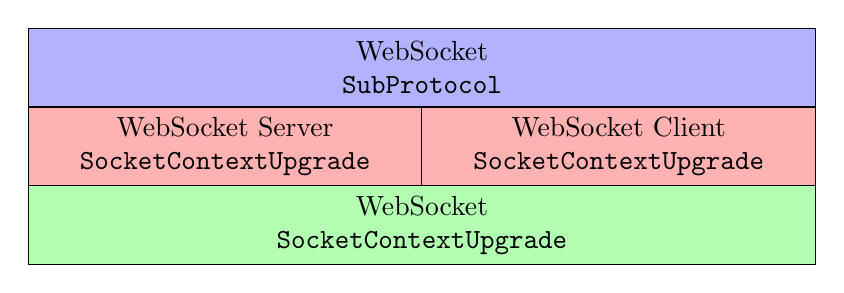
\begin{tikzpicture}
        \draw node [outer sep=0, inner sep=0, draw, fill=green!30, minimum width=10cm, minimum height=1cm, align=center] (wstr) {WebSocket\\\texttt{SocketContextUpgrade}};
        \draw (wstr.north) node[anchor=south west, outer sep=0, inner sep=0, fill=red!30, draw, minimum width=5cm, minimum height=1cm, align=center] (wsc) {WebSocket Client\\\texttt{SocketContextUpgrade}};
        \draw (wstr.north) node[anchor=south east, outer sep=0, inner sep=0, fill=red!30, draw, minimum width=5cm, minimum height=1cm, align=center] (wss) {WebSocket Server\\\texttt{SocketContextUpgrade}};
        \draw (wss.north east) node[anchor=south, outer sep=0, inner sep=0, fill=blue!30, draw, minimum width=10cm, minimum height=1cm, align=center] (sp) {WebSocket\\\texttt{SubProtocol}};
      \end{tikzpicture}
      \caption{WebSocket application protocol in detail}
    \end{figure}
  \end{center}
\begin{itemize}
     \item The WebSocket libraries are loaded dynamically (\texttt{dlopen()}, \ldots) during an HTTP \texttt{upgrade}.
     \item Using the requested sub-protocol (e.g. \texttt{tiktaktoe}, \texttt{echo}, \texttt{mqtt}) the corresponding \texttt{SubProtocol} library is dynamically loaded.
     \item Both WS libraries and sub-protocol (SP) Libraries must obey a naming convention in order to be found.
     \item WS and SP libraries must provide \texttt{static} factory-factory functions.
     \item SP libraries must be implemented by the user (abstract base class \texttt{SubProtocol).}
   \end{itemize}
\end{frame}
